\chapter{Wykorzystane technologie (AK i JC)}
\label{ch:technologies}

% setup
\graphicspath{{2_technologies/static/}}

% content
W niniejszym rozdziale zawarty został opis stosowanych przez autorów pracy technologi. Przedstawione informacje obejmują zarówno wykorzystane języki programowania, jak również narzędzia, których zadaniem jest ułatwienie tworzenia wysokiej jakości kodu źródłowego, czy też automatyzacja procesów zachodzących na różnych etapach cyklu życia oprogramowania. Niniejszy rozdział stanowi krótkie wprowadzenie do każdego z omawianych zagadnień - zaawansowane aspekty każdej z opisywanych technologii przedstawione zostały w dalszej części pracy, podczas omawiania konkretnych, osiągniętych za ich pomocą, rozwiązań. 


\section{Język C++ (AK)}
C++ to stworzony w latach 80-tych XX wieku wszechstronny język programowania, oryginalnie mający stanowić rozszerzenie popularnego języka C o mechanizmy pozwalające na programowania obiektowe. Wraz z jego rozwojem pojawiło się natomiast wsparcie dla innych paradygmatów programowania, dzięki czemu nowoczesny C++ pozwala stosować (poza paradygmatem proceduralnym oraz obiektowym) programowanie funkcyjne oraz generyczne. Z tego też powodu język ten znajduje współcześnie bardzo szerokie zastosowanie, od rozwiązań telekomunikacyjnych po oprogramowanie dla eksperymentów fizycznych, takich jak detektor ATLAS w CERN. Jest on ponadto bardzo istotny z punktu widzenia niniejszej pracy, ponieważ za jego pomocą napisana została większość oprogramowania systemu GGSS.

C++ jest wydajnym językiem kompilowanym, opartym o statyczne typowanie. Udostępnia mechanizmy pozwalające programiście na działanie na wielu poziomach abstrakcji - możliwe są zarówno niskopoziomowe operacje, takie jak manualne zarządzanie pamięcią, jak również modelowanie wysokopoziomowej logiki biznesowej. W ciągu ostatnich dziesięciu lat miał miejsce szczególnie intensywny rozwój języka, czego początek stanowi pojawienie się przełomowego standardu C++11. Od tego czasu regularnie, co trzy lata, wydawana jest nowa wersja standardu języka, a zatem od 2011 roku pojawiły się następujące wydania:
\begin{itemize}
\item C++11 - uznawane za przełomowe, zawiera modyfikacje w znacznym stopniu zmieniające sposób tworzenia oprogramowania w języku C++. Wprowadzone zostały zarówno rozszerzenia w rdzeniu języka, jak i w bibliotece standardowej. Najważniejsze elementy standardu C++11 to m.in.: semantyka przenoszenia i referencje do \emph{r-wartości}, wyrażenia lambda, słowa kluczowe \lstinline{override} i \lstinline{final} ułatwiające programowanie obiektowe, inferencja typów za pomocą słowa kluczowego \lstinline{auto}, wsparcie dla wielowątkowości (model pamięci oraz funkcjonalności w bibliotece standardowej), tzw. inteligentne wskaźniki (ang. \emph{smart pointers}) ułatwiające zarządzanie pamięcią czy nowe kontenery biblioteki standardowej.
\item C++14 - mniejsze wydanie, stanowiące uzupełnienie standardu C++11 o pomniejsze funkcjonalności oraz poprawki. Wprowadzone zmiany to m.in. ułatwienia w korzystaniu ze słowa kluczowego \lstinline{constexpr} oraz generyczne wyrażenia lambda. 
\item C++17 - wprowadza wiele nowych funkcjonalności, m.in. bibliotekę do obsługi systemu plików, typ \lstinline{std::optional} czy możliwość wykonania inicjalizacji w wyrażeniu warunkowym
\item C++20 - najnowsze wydanie języka, pod względem liczby wprowadzonych zmian większe od dwóch poprzednich. Przykładowe elementy tego standardu to: koncepty (ang. \emph{concepts}), moduły czy biblioteka pozwalająca na operacje na zakresach (ang. \emph{ranges}).
\end{itemize}

Obecnie trwają pracę nad nowym standardem języka, którego publikacja planowana jest na rok 2023. Poza wprowadzaniem funkcjonalności, nowe wydania języka C++ eliminują te elementy języka, które uznawane są za przestarzałe. Przykładem może być obecny w bibliotece standardowej od wczesnych wersji języka inteligentny wskaźnik \lstinline{std::auto_ptr} - został on oznaczony jako przestarzały (ang. \emph{deprecated}) po pojawieniu się nowych rozwiązań w standardzie C++11, a następnie został usunięty z języka wraz z wprowadzeniem standardu C++17. Tego typu zmiany mają na celu wspieranie tzw. \emph{dobrych praktyk} - zasad ułatwiających tworzenie łatwego w utrzymaniu i rozwoju oprogramowania (np. poprzez odpowiednie zarządzanie zasobami).

Z punktu widzenia niniejszej pracy szczególnie istotne są zmiany wprowadzone w standardzie C++11 - z uwagi na ograniczenia w środowisku docelowym systemu GGSS jest to najnowsze dostępne tam wydanie języka (więcej informacji na ten temat przedstawione zostanie w dalszej części pracy). Dlatego też zaprezentowany zostanie krótki przykład obrazujący część funkcjonalności wprowadzonych właśnie w tym standardzie. W przykładzie tym zaimplementowana została prosta hierarchia klas reprezentujących zasilacze: jedna abstrakcyjna klasa bazowa \lstinline{PowerSupply} oraz dwie implementacje: \lstinline{CaenPowerSupply} oraz \lstinline{MockPowerSupply}. W funkcji \lstinline{main()} tworzony i wypełniany jest kontener przechowujący wskaźniki zawierające adresy obiektów reprezentujących różne typy zasilaczy. Następnie dla każdego z istniejących zasilaczy następuje polimorficzne wywołanie metody pozwalającej na zmianę wartości zasilania (tutaj powoduje jedynie wypisanie odpowiedniej wiadomości na standardowe wyjście). Celem przykładu jest zaprezentowanie prostego scenariusza, w którym nowe funkcjonalności języka wpływają pozytywnie na jakość i bezpieczeństwo kodu - nie prezentuje więc on w sposób bezpośredni zaawansowanych elementów języka (takich jak możliwość metaprogramowania za pomocą szablonów).

Na listingu \ref{lst:cpp_old} przedstawiona została implementacja przykładu zgodna ze standardem C++03. Najważniejsze cechy zaprezentowanego kodu, charakterystyczne dla kodu źródłowego powstającego przed pojawieniem się standardu C++11, to: 
\begin{itemize}
\item konieczność manualnego zarządzania pamięcią - widoczne zastosowanie operatora \lstinline{delete} pod koniec funkcji \lstinline{main()}
\item brak bezpośredniej możliwości zadeklarowania klasy jako \emph{finalna} - tzn. taka, po której nie można dziedziczyć (przed standardem C++11 istniały jednak techniki, wykorzystujące zaawansowane funkcjonalności języka, pozwalające osiągnąć podobny rezultat - ze względu na stopień skomplikowania nie zostały tu jednak zaprezentowane)
\item brak możliwości wskazania, że metoda w klasie pochodnej nadpisuje (ang. \emph{override}) metodę wirtualną z klasy bazowej
\item rozbudowana, nieczytelna składnia pętli \lstinline{for} operującej na kontenerze za pomocą iteratora 
\end{itemize}

\lstinputlisting[
    language=C++, 
    caption={Przykładowa implementacja prostej hierarchii dziedziczenia oraz polimorficznego wykonania metody - standard C++03. Należy zwrócić uwagę na konieczność manualnego zarządzania pamięcią oraz brak możliwości wskazania, że metoda w klasie pochodnej nadpisuje metodę wirtualną z klasy bazowej.}, 
    label={lst:cpp_old}
]{2_technologies/code_samples/cpp_example_old.cpp}


Na listingu \ref{lst:cpp_new} przedstawiona została natomiast implementacja przykładu za pomocą języka C++ w standardzie 11. Najważniejszą zmianą jest zastosowanie inteligentnego wskaźnika \lstinline{std::unique_ptr<PowerSupply>}, automatyzującego zarządzanie wskazywanym zasobem (pamięć zostaje zwolniona, gdy wskaźnik ulega destrukcji). Powoduje to, że programista nie jest odpowiedzialny za manualne sprawowanie kontroli nad pamięcią, a co za tym idzie zmniejsza prawdopodobieństwo wystąpienia związanych z tym błędów (takich jak wycieki pamięci). Kolejną zmianą jest zastosowanie słowa kluczowego \lstinline{override} w celu zadeklarowania, że metoda w klasie pochodnej (np. \lstinline{CaenPowerSupply}) nadpisuje metodę z klasy bazowej (tutaj \lstinline{PowerSupply}). W przypadku, gdy powyższe nie jest prawdą (np. za sprawą błędnej pisowni lub braku słowa kluczowego \lstinline{const}), kompilator zgłosi błąd. W klasach pochodnych zastosowane zostało ponadto słowo kluczowe \lstinline{final}, powodujące, że po klasach tych nie można dziedziczyć - jego stosowanie może wynikać m.in. z zalecenia mówiącego, że dziedziczenie powinno być możliwe jedynie w przypadku klas, które są z myślą o nim projektowane (np. klasy abstrakcyjne). Wymienione powyżej zmiany, możliwe dzięki stosowaniu funkcjonalności nowoczesnego języka C++, pozwalają na zwiększenie niezawodności tworzonego kodu źródłowego, m.in. poprzez zabezpieczenie go przed prostymi błędami oraz dostarczenie dodatkowej, wbudowanej wprost w język, dokumentacji. Innym typem zmiany, nastawionym w większym stopniu na zwiększenie czytelności kodu, jest natomiast zastosowanie w przykładzie pętli zakresowej do iteracji po kontenerze oraz wykorzystanie słowa kluczowego \lstinline{default} w deklaracji domyślnego destruktora wirtualnego klasy bazowej. W standardzie C++11 wprowadzonych zostało znacznie więcej podobnych udoskonaleń, a ponadto wprowadzone zostały mechanizmy ułatwiające optymalizację oprogramowania (np. ze względu na szybkość wykonania lub ilość zużytej pamięci) - jednak ze względu na konieczność zachowania prostego charakteru przykładu nie zostały one zaprezentowane.

\lstinputlisting[
    language=C++, 
    caption={Przykładowa implementacja prostej hierarchii dziedziczenia oraz polimorficznego wykonania metody - standard C++11. Widoczne zastosowanie słów kluczowych \lstinline{default}, \lstinline{final} oraz \lstinline{override}, pętli zakresowej oraz inteligentnego wskaźnika.}, 
    label={lst:cpp_new}
]{2_technologies/code_samples/cpp_example_new.cpp}

\clearpage
Język C++ charakteryzuje się ponadto istnieniem dodatkowych, nie będących częścią standardu, bibliotek poszerzających zestaw dostarczanych przez niego narzędzi. Z punktu widzenia systemu GGSS istotne są: zestaw bibliotek Boost, biblioteka GNU Scientific Library (GSL) oraz zestaw bibliotek i narzędzi Qt.

Boost to popularna kolekcja bibliotek dla języka C++, ułatwiająca wiele aspektów tworzenia oprogramowania poprzez dostarczenie zróżnicowanego zestawu narzędzi programistycznych: zarówno ogólnego przeznaczenia, jak i bardzo wyspecjalizowanych. Pakiet Boost rozwijany jest znacznie szybciej niż biblioteka standardowa języka C++, a ponadto niektóre jego elementy stanowiły podstawę dla funkcjonalności dodawanych do języka w nowych jego wydaniach (np. wprowadzona w standardzie C++17 biblioteka \lstinline{filesystem}, służąca do zarządzania systemem plików, oparta jest na analogicznym module z zestawu Boost). Przykładowe funkcjonalności udostępniane przez pakiet Boost to: rozszerzona względem biblioteki standardowej obsługa łańcuchów znakowych, dodatkowe kontenery (np. \lstinline{Boost.MultiIndex}), implementacja algorytmów grafowych czy asynchroniczne programowanie sieciowe. Ze względu na szeroki zakres oferowanych funkcjonalności, pakiet Boost stosowany jest również przez warstwę oprogramowania omawianego w niniejszej pracy systemu GGSS.

GNU Scientific Library (GSL) to napisana w języku C biblioteka udostępniająca narzędzia programistyczne do wykonywania obliczeń numerycznych. Pozwala na wykonywanie operacji takich jak: znajdowanie miejsc zerowych funkcji, dopasowywanie krzywej do danych czy całkowanie metodą Monte Carlo. Ze względu na drugą z wymienionych tu funkcjonalności biblioteka ta znalazła zastosowanie w oprogramowaniu systemu GGSS.

Qt jest zestawem narzędzi programistycznych umożliwiających tworzenie przenośnych aplikacji okienkowych z wykorzystaniem języka C++. Technologia ta nie została zastosowana w rdzeniu oprogramowania systemu GGSS, natomiast przy jej pomocy stworzone zostały pomniejsze narzędzia wchodzące w skład projektu. Opisane w niniejszej pracy rozwiązania nie są oparte o Qt, dlatego też szczegółowy opis dostarczanych przez zestaw narzędzi nie zostanie w niej zamieszczony.


\section{Język Python (AK)}
Python jest opartym na dynamicznym systemie typów językiem programowania ogólnego przeznaczenia, charakteryzującym się bardzo szerokim obszarem zastosowań, obejmującym m.in. automatyzację za pomocą skryptów, tworzenie aplikacji internetowych czy eksplorację danych. Cechą najczęściej kojarzoną z tym językiem jest intuicyjna składnia, ułatwiająca zarówno jego naukę, jak i zrozumienie napisanych z jego pomocą programów. Python jest językiem wieloparadygmatowym, pozwalającym pisać zarówno w sposób proceduralny, jak i obiektowo i funkcyjnie. W systemie GGSS język ten stosowany jest jako narzędzie pomocnicze, rozumiane przede wszystkim jako język skryptowy wykorzystywany do tworzenia infrastruktury projektu.

Obecnie język Python istnieje w dwóch szeroko stosowanych wersjach: Python 2 oraz Python 3. Oficjalnie wspieraną wersją jest wydanie trzecie (wsparcie dla Pythona w wersji drugiej zakończone zostało na początku 2020 roku), w rzeczywistości jednak, ze względu na fakt, iż wersje te nie są ze sobą w pełni kompatybilne, oprogramowanie napisane za pomocą Pythona 2 wciąż znaleźć można w wielu projektach. Z punktu widzenia systemu GGSS różnice między tymi wydaniami nie są w dużym stopniu znaczące (ponieważ język ten używany jest jako pomocnicze narzędzie), jednakże preferowana jest wersja trzecia.

Na listingu \ref{lst:python} przedstawiony został prosty przykład zastosowania języka Python jako narzędzia do tworzenia skryptów. W tym przypadku jest to prosty skrypt, generujący sto pierwszych elementów ciągu Fibonacciego i zapisujący je do pliku tekstowego w postaci kolumny. Przykład obrazuje wykorzystanie takich elementów języka jak generatory, pętle oraz operacje na plikach.


\lstinputlisting[
    language=Python, 
    caption={Przykładowy skrypt napisany w języku Python, którego działanie polega na wygenerowaniu stu pierwszych elementów ciągu Fibonacciego i zapisaniu otrzymanego wyniku do pliku tekstowego.}, 
    label={lst:python}
]{2_technologies/code_samples/python_example.py}


\section{Narzędzia do analizy oprogramowania (AK)}
Wraz z postępującym rozwojem szeroko rozumianej informatyki, stale rośnie złożoność powstającego oprogramowania. Powoduje to, że utrzymanie wysokiej jakości kodu źródłowego staje się coraz trudniejsze, a w przypadku wielu projektów - niemożliwe do realizacji bez pomocy dodatkowych narzędzi. Niniejsza część pracy magisterskiej stanowi krótkie wprowadzenie do szerokiej tematyki, jaką jest analiza oprogramowania. Przedstawione zostaną podstawy teoretyczne, jak również zarysowane zostanie działanie narzędzi wykorzystywanych przez autorów podczas prac nad systemem GGSS. Ze względu na charakter projektu, omówione zostaną wyłącznie technologie pozwalające na pracę z oprogramowaniem napisanym w językach C i C++. 

\subsubsection*{Wstęp teoretyczny}
Pojęcie \emph{narzędzi do analizy oprogramowania} definiuje bardzo szeroki zakres różnego rodzaju programów, umożliwiających lub ułatwiających wykonywanie działań takich jak: znajdowanie i eliminowanie błędów oraz przyczyn ich występowania, badanie zużycia różnego rodzaju zasobów (np. pamięci) oraz analiza jakości kodu źródłowego. W zależności od przyjętego kryterium podziału, analizę oprogramowania kategoryzować można na zróżnicowane sposoby. Jeśli zatem podział następować ma na podstawie tego, kiedy analiza jest przeprowadzana, to wyróżnić można następujące jej rodzaje:
\begin{itemize}
    \item analiza statyczna (ang. \emph{static analysis}) - następuje bez uruchamiania badanego programu. Przykładem narzędzi umożliwiających wykonywanie tego typu badań są tzw. lintery (ang. \emph{linter}), pozwalające na analizę kodu źródłowego pod względem stylu programowania i umożliwiające wczesne wykrywanie wielu błędów.
    \item analiza dynamiczna (ang. \emph{dynamic analysis}) - następuje w trakcie wykonania programu. Jako przykład oprogramowania wykonującego tego typu analizę podać można narzędzia umożliwiające tzw. profilowanie (ang. \emph{profiling}), pozwalające na monitorowanie wydajności i zużycia zasobów przez badany program.
\end{itemize}

Inne kryterium podziału ... 


\subsubsection*{Valgrind}


\subsubsection*{Statyczna analiza kodu źródłowego}


\subsubsection*{Podsumowanie}

% Wstep teoretyczny - czym jest analiza kodu, jakie mamy rodzaje, co to jest instrumentacja
% Omowienie Valgrinda jako frameworka, wskazanie narzedzia Memcheck
% Krotkie omowienie dzialania Memcheck, m.in. rodzaje wyciekow pamieci, jakie są ich konsekwencje, wskazac te potencjalnie grozne dla aplikacji dzialajacych jako uslugi (stopniowe nagromadzenie sie zuzytej pamieci - przyklad)
% Krotko o innych narzedziach (np. Cachegrind), czemu tutaj mniej istotne
% Statyczna analiza kodu źródłowego - jakie możliwości daje CLion oraz clang-tidy
% Wskazac mozliwości zastosowania analizy w wiekszym srodowisku (np. SonarLint i SonarQube w wielu firmach), możliwość wlaczenia takiego rozwiazania w CI + dlaczego u nas tego nie ma

\section{System kontroli wersji Git (JC)} % submoduly, repozytoria, gałęzie %
Git jest to oprogramowanie służące do śledzenia zmian dokonywanych w zadanym zbiorze plików. Głównym celem jest umożliwianie sprawnej współpracy między programistami podczas procesu wytwarzania oprogramowania. Narzędzie to pozwala m.in. na równoległa pracę nad jednym zestawem plików przez wielu deweloperów, wersjonowanie zmian wprowadzanych w projekcie. Cechą wyróżniającą technologię Git od pozostałych rozwiązań służących do śledzenia zmian jest prędkośc działania, możliwość zastosowania wielu podejść dotyczących przepływu pracy (ang. \emph{workflow}), czy też ilość kopii zapasowych, automatycznie tworzących się w ramach korzystania z wyżej wymienionego narzędzia.

Podstawowym i najważniejszym elementem technologii Git są tak zwane repozytoria (ang. \emph{repository}). U swojej podstawy jest to ukryty folder \lstinline{.git}, który jest tworzony w momencie aktywowania kontroli wersji w projekcie. Folder ten znajduje się w głównej ścieżce projektu, czyli \lstinline{<ścieżka do projektu>/.git}. Zawarte są w nim wszystkie informacje niezbędne do poprawnego działania technologii Git, np.: informacje o zmianach w prowadzonych w plikach z każdą rewizją (ang. \emph{commit}), wszystkie informacje na temat gałęzi (ang. \emph{branches}) w projekcie, informacje o zmianach lokalnych oraz o etapie (ang. \emph{stage}) w jakim się znajdują. Takie repozytorium wraz z samą zawartością projketu możemy zdeponować w jednym z portali obsługujących technologię git, na przykład: portal GitLab.

Chcąc utrwalić zmiany w kodzie wykorzystując technologię Git należy skorzystać z funkcjonalności rewizji. W pierwszej kolejności należy dodać pliki, których stan ma być zachowany za pomocą komendy \lstinline{git add}, a następnie wykonując komendę \lstinline{git commit} należy utworzyć nową rewizję. W ten sposób utworzona rewizja posiada swój własny, unikalny identyfikator, korzystając z niego możemy w dowolnym momencie wrócić wszystkie pliki do stanu w którym znajdowały się w trakcie tworzenia wyżej wymienionej rewizji. Rewizję taką możemy również umieścić na zdalnym repozytorium utrzymywanym w ramach wcześniej wspomnianych portali.

Bardzo przydatną funkcjonalnością Git, szczególnie w przypadku równoległej pracy nad tymi samymi plikami, jak i utrzymywania porządku, są tak zwane gałęzie. Pozwalają one na utworzenie alternatywej historii rewizji, dzięki czemu deweloperzy mogą prowadzić w pełni odseparowaną pracę nad funkcjonalnościami. W momencie, gdy zakończą oni pracę mogą połączyć swoje gałęzie w jedną, która będzie zawierałą wszystkie przez nich wykonane zmiany. W przypadku wystąpienia zmian konfliktujących ze sobą, np.: zmiana tej samej linijki kodu na obydwu gałęziach, należy problem taki rozwiązać ręcznie, to znaczy programista musi ręcznie wybrać wersję danej linijki kodu, która jest odpowiednia, bądź ręcznie połączyć obie wersje w jedną.

Jedną z bardziej zaawansowanych funkcji Git, która została mocno wykorzystana w projkecie są submoduły (ang. \emph{submodules}). Pozwalają one na powiązanie dwóch niezależnych repozytoriów. W repozytorium nadrzędnym należy wykonać komendę \lstinline{git submodule add <url>}. Powoduje ona dodanie innego, zewnętrznego repozytorium jako podkatalog w repozytorium nadrzędnym. Wytwarzanie nowych rewizji w repozytorium nadrzędnym, oprócz zapisania stanu plików w tymże repozytorium, skutkuje zachowaniem informacji o identyfikatorze rewizji submodułu. Dzięki temu jesteśmy w stanie wersjonować zarówno nasze pliki, jak i wersję zależności z których korzystamy. Dodatkowo wykorzystując submoduły Git pozwala na bardzo prostą inicjalizację projektu składającego się z wielu repozytoriów, czy też zarządzanie nim.
%https://git-scm.com/
\section{Portal GitLab (JC)}

GitLab jest to serwis hostujący repozytoria Git oparty o gui (\emph{graphical user interface}) w postaci portalu internetowego. Zadaniem tego rozwiązanie jest możliwość przechowywania oraz udostępniania repozytoriów Git. Rysunek \ref{fig:gitlab} przedstawia panel grupy w ramach platformy GitLab oraz kilka repozytoriów w ramach niej zawartych.

\begin{figure}[H]
    \centering
    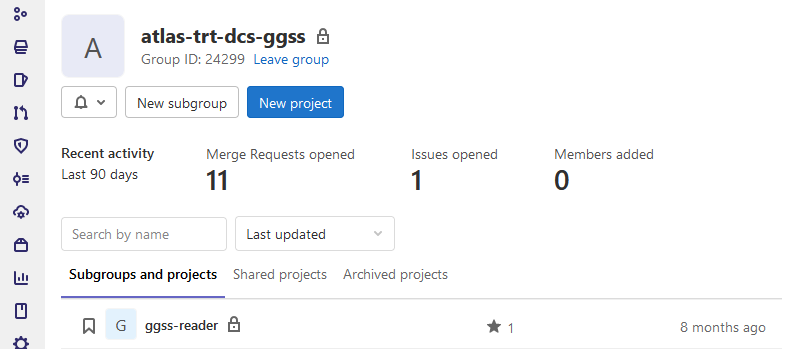
\includegraphics[width=0.80\textwidth]{gitlab}
    \caption{Panel grupy na paltformie GitLab}
    \label{fig:gitlab}
\end{figure}

Oprócz tego portal ten wzbogaca współpracę opartą na repozytoriach poprzez wprowadzenie tak zwanych \emph{merge request}. Pozwalają one na współpracę nad łączeniem dwóch gałęzi repozytorium w jedno. Rysunek \ref{fig:merge} przedstawia część przykładowego panelu \emph{merge request}. Oprócz logu wydarzeń widoczne są informację na temat: osoby, która zatwierdziła zmiany, statusu skonfigurowanej automatyzacji, czy też stanu danego merge request. Dostępne są również zakładki, gdzie sprawdzić można wszystkie rewizje które wchodzą w skład gałęzi, którą chcemy dołączyć oraz różnice we wszystkich zmienionych plikach.

\begin{figure}[H]
    \centering
    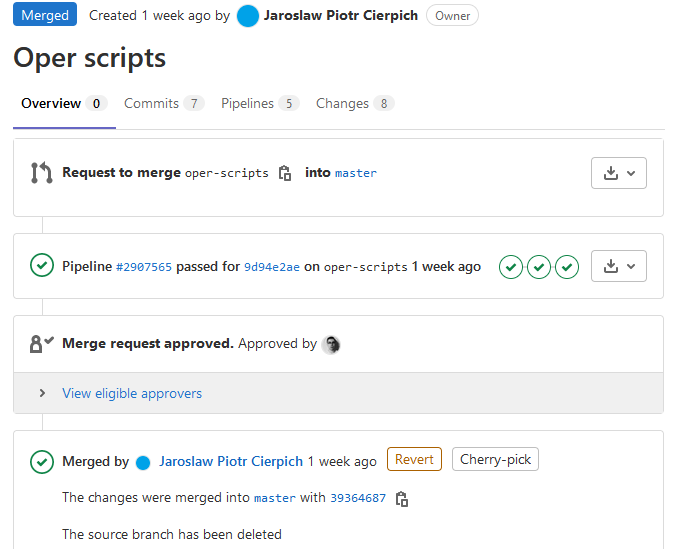
\includegraphics[width=0.85\textwidth]{gitlab_merge}
    \caption{Przykładowy \emph{merge request} na platformie GitLab}
    \label{fig:merge}
\end{figure}

Wraz ze wzrostem portali takich jak GitLab zaczęto wprowadzać dodatkowe udogodnienia dla programistów, które szczególnie skupiają się na procesie wytwórczym kodu, infrastrukturze do tego stosowanej oraz różnym praktykom stosowanym w nowoczesnych projektach. Jedną z takich funkcjonalności jest \emph{GitLab CI/CD}, czyli część portalu GitLab oraz framework pozwalający na automatyzację procesu wytwórczego poprzez zastosowanie podejścia Continuous Integration/Continuous Delivery. Gitlab CI/CD pozwala na zdefiniowanie akcji, które mają być wykonywane automaczynie, w przypadku wystąpenia pewnych zdarzeń, na przykład: automatycznie wykonanie testów w momencie utworzenia nowej rewizji repozytorium na portalu Gitlab, czy też utworzenie nowego wydania aplikacji po przekazaniu odpowiedniego tag'a do repozytorium na platformie.

Wszystkie akcje zawarte w wyżej wymienionej automatyzacji wykonywane są na specjalnie przygotowanych maszynach wirtualnych zarejestrowanych w portalu Gitlab, czyli \emph{Gitlab Runners}. Maszyny te posiadają zainstalowane odpowiednie rozszerzenia oraz oprogramowanie \emph{docker}, ponieważ większość akcji wykonywana jest w ramach kontenerów.

%https://en.wikipedia.org/wiki/GitLab
\section{Narzędzie CMake (AK)}
% Krotki opis co to jest, czym sie rozni od Make, zalety
% Opis dwoch wersji, jakie sa roznice miedzy nimi
% Prosty przyklad
% Co to jest CPack i CTest, do czego sluza


\section{Menadżer pakietów RPM (JC)}
\emph{RPM Package Manager} jest systemem do zarządzania pakietami na systemach z rodziny Red Hat, Fedora, CentOS, OpenSUSE. Posługuje się on pakietami z rozszerzeniem \emph{.rpm}. W ramach takiego pakietu zawarte są:
\begin{itemize}
    \item główna zawartość - na przykład: skompilowana aplikacja, gotowy skrypt bash, itp.
    \item metadane - informacje o autorze, zawartości, wersji zawartości, opis pakietu, wymagane zależności
    \item logika instalacji oraz logika dezinstalacji - skrypty mające na celu przygotowanie systemu do instalacji oraz posprzątanie systemu po dezinstalacji pakietu
\end{itemize}

Instalacja oprogramowania za pomocą menadżera pakietów pozwala na znacznie przyspieszenie procesu. Zazwyczaj wszystkie akcje, które są wymagane przed zainstalowaniem oprogramowania, wykonywane są w ramach logiki instalacji. Menadżer pakietów, wykorzystując zewnętrzne repozytoria, jest w stanie pobrać i zainstalować wszystkie pakiety jakich wymaga przez nas instalowany pakiet. Dodatkowo menadżer pakietów RPM zapewnia zabezpiecznie i weryfikacje poprawności pakietu w postaci technologii \emph{GPG} oraz  \emph{MD5}.

%https://rpm.org/documentation.html
%https://en.wikipedia.org/wiki/RPM_Package_Manager